\chapter{Used algorithms and key concepts}
This section offers basic introduction to multiple state-of-the-art algorithms used in this work. It starts with explanation of graph-based SLAM variant. Next section \ref{sec:map_alg} describes \gls{NDT} based map representations. Section \ref{sec:reg_alg} is dedicated to \gls{NDT} based registration algorithms. We also include basic introduction to \gls{ICP} and Correlative registration algorithm.   

\section{Graph-based SLAM}
\label{sec:graph_base_slam}
A graph-based SLAM solves SLAM pose estimation problem by constructing graph representation. This graph is commonly called a pose graph. Nodes of the graph represent potential poses of robot at certain time stamp $ T $. Therefore, nodes are representing our trajectory $ \{\textbf{x}_{1},...,\textbf{x}_{T}\} $. Nodes also hold state of the current map. Edges in the graph represent possible spatial transformation between nodes. Edge is generated out of noisy sensor data. Therefore, we need to model uncertainty of this movement. It is represented by probability distribution and included in the edge. Generation of constrains is done by algorithm's front-end. It creates them either from odometry $  \textbf{u}_{T} $ or by measurement data  $ \textbf{z}_{T} $ registration. Once the graph is completed ,it is optimized by algorithms back-end. Result of this process is the most likely position of all nodes in the graph.

\subsection {Pose graph creation}
\label{Pose_graph_creation}
Process of graph creation operates in \gls{SLAM}'s front-end. First step is to receive robot's movement. This transformation may come from wheels' encoders, visual odometry from camera or \gls{IMU}. Front-end also receives a covariance of the transformation based on noise model of source sensor. From transformation and covariance we can create an edge for the graph. This edge type is usually called odometry edge. Consecutive odometry measurements creates long chain of edges in graph.

Nodes represent current robot position. Therefore, they should have some initial estimate. This initial guess may come from concatenation of transformations in odometry edges. Another method is to use propagation of transformation through minimum spanning tree constructed out of full graph. 

Second type, represents edges from nodes to landmarks. A landmark is and unique descriptors of the place. When landmark is detected, front-end creates node representing this place and landmark edge connecting it with graph. Edge carries transformation between current node and landmark. If landmark already exists than created edge might help to optimize correct pose estimate of other nodes.

   
Third common type of edges are loop closure edges. These edges usually connect two nodes, which share same perception of the world. Aligning these perceptions yields virtual transformation between these nodes. A covariance needs to be provided from alignment process and depends on used technique. Loop closure edge usually exists if we have revisited same place again. This is crucial information for \gls{SLAM}'s back-end. Based on it optimalization finds out if odometry edges reliably represent reality and adjust pose estimates.

\subsection {Loop closure creation}
\label{subsec:loop_closure_creation}
First step of correct loop closure creation is to identify all nodes ,which might have overlapping measurements. Given pose $a$ we find all nodes $b_{1} ... b_{n}$ from graph whose sensor measurements overlap pose $a$. This could be determined by finding relative position of nodes $a$ and $b_{i}$. One possible method how to determine is to use Dijkstra projection mentioned in \cite{Olson2009Loop}. Dijkstra projection starts at node $a$ and concatenate covariances and transformation along the minimum uncertainty path. This path is selected based on determinant of covariance matrix. Small covariance matrix has lower determinant than covariance matrix with large numbers. Minimum uncertainty selection guaranties that algorithm will get to the target $b_{i}$ with maximum precision. Concatenation of covariances is done based on equation:
\begin{equation}
P_{a+b} = J_{a} P_{a} J_{a}^{T} + J_{b} P_{b} J_{b}^{T}
\end{equation}   
\begin{equation}
J_{a} = 
\begin{pmatrix}
1 & 0 & -x\sin\theta -y\cos\theta  \\
0 & 1 & x\cos \theta  - y\sin\theta  \\
0 & 0 & 1
\end{pmatrix} 
J_{b} = 
\begin{pmatrix}
\cos\theta & -\sin\theta & 0  \\
\sin\theta & \cos\theta & 0\\
0 & 0 & 1
\end{pmatrix} 
\end{equation} 
where $P_{a}$ is acumulated covariance, $P_{b}$ is aditional covariance, Jaccobian $J_{a}$ use parameters from transformation $(x,y,\theta)_{a}$ and $J_{b}$ from  $(x,y,\theta)_{b}$ Concatenation of transformations is defined as:
\begin{equation}
\label{eq:concat_trans}
\begin{pmatrix}
x \\ y
\end{pmatrix}_{a+b}
=
\begin{pmatrix}
x \\ y
\end{pmatrix}_{a}
+ R(\theta_{a}) 
\begin{pmatrix}
x \\ y
\end{pmatrix}_{b}
\end{equation}
\begin{equation}
\theta_{a+b} = \theta_{a} + \theta_{b}
\end{equation}
where $R(\theta_{a})$ is rotation matrix created from angle $\theta_{a}$.

After successful generation of overlapping nodes, every potential pair needs to be tested by registration algorithm. This algorithm needs to be robust enough to reject as many incorrect pairs as possible. If matching is possible it should align measurements and return best transformation. More about this type of algorithms can be found in section \ref{Scan_reg}.

Even the best registration algorithm may fail and return erroneous measurement. Loop closure process needs to reject these errors. One solution is to use method proposed by \cite{Olson2009Loop}. In this approach we first group loop closure edges into groups based on their topological distance from each other. Later we validate every cluster against internal inconsistencies. Edges marked as inconsistent are deleted from system. 

Other option is to use robust optimization engines, witch can identify outliers in the form of error edges. Comparison of known outliers rejection methods was done by \cite{RobustOpt}. 


\newpage

\subsection{Optimization}
Back-end receives graph with odometry edges and loop closure edges. The main task of back-end is to optimize this graph and return the most likely position of nodes. Popular method of optimization is to use the Gauss-Newton or the Levenberg-Marquardt algorithms. 

To utilize these methods we first need to define our error function. We will use notation similar to one presented in section \ref{sec:SLAM_def}. Let $\textbf{x} = (\textbf{x}_{1},...,\textbf{x}_{T})^{T} $ be a vector of graph's nodes positions. Let $z_{i,j}$ to be a registration algorithm transformation between nodes $x_{i}$ and $x_{j}$. Let $\Omega_{i,j}$ be a information matrix of this transformation (information matrix is an inverse of covariance). Lastly let $\hat{z}_{i,j}$ be a estimate of registration transform received from initial configurations of nodes i and j.

The log-likelihood of measurement $z_{i,j}$ is than defined as:
\begin{equation}
l_{i,j} = (\hat{z}_{i,j} - z_{i,j})^{T} \Omega_{i,j} (\hat{z}_{i,j} - z_{i,j}) 
\end{equation}  
where $(\hat{z}_{i,j} - z_{i,j})$ is a difference between expected measurement and real measurement. Now we can define out error function as

\begin{equation}
F(\textbf{x}_{1,T}) = \sum_{<i,j>\in G}^{} (\hat{z}_{i,j} - z_{i,j})^{T} \Omega_{i,j} (\hat{z}_{i,j} - z_{i,j}) 
\end{equation}

Our goal is to calculate such a $\textbf{x}$ that this function is minimal. More formaly we wan to find solution to
\begin{equation}
\bar{x}_{1,T} = argmin_{\textbf{x}} \ F(\textbf{x})
\end{equation}

 Information on how to minimize this function, calculate derivatives and how to exploit structure of the problem to get significant speed gains continue in reading in this tutorial \cite{GraphTutorial}.

\newpage


\section{NDT mapping algorithms}
\label{sec:map_alg}
\subsection{NDT grid}
\label{subsec:NDT_grid}
\gls{NDT} grid representation was first time used by \cite{Biber03} in their scan registration process. Central idea was to convert laser scan into grid with cells containing normal distributions. Points in space from laser scanner are first separated into corresponding cells. From points in single cell we approximate normal distribution $(\mu_{i},P_{i})$ by calculating mean and covariance:
\begin{equation}
\mu_{i} = \dfrac{1}{n}\sum_{k=1}^{n}x_{k}
\end{equation}  
\begin{equation}
P_{i} = \dfrac{1}{n-1}\sum_{k=1}^{n}(x_{k}-\mu_{i})(x_{k}-\mu_{i})^{t}
\end{equation} 
\gls{NDT} grid was than used for registration.Originally proposed grid could be updated with new laser scans only by keeping used points and recalculating all cells again. This has changed with proposed recursive covariance update step by \cite{Saarinen13}. Their update step offers way how to fuse in new measurements. First it calculate normal distributions for added points. In second step, it merges old covariances with new one.

Consider two sets of measurement $\{x_{i}\}^{m}_{i=1}$ and $\{y_{i}\}^{n}_{i=1}$ than formula for mean calculation is in equation \eqref{NDT_mean_RCU}. \gls{RCU} is in equation \eqref{NDT_covar_RCU}
\begin{equation}
T_{x} = \sum_{i =1}^{m}x_{i} \quad
T_{y} = \sum_{i =1}^{n}y_{i} \quad
T_{x\oplus y} = T_{x} + T_{y} 
\end{equation}

\begin{equation}
\label{NDT_mean_RCU}
\mu_{x\oplus y} =\dfrac{1}{m + n}T_{x\oplus y}
\end{equation} 

\begin{equation}
S_{x} = \sum_{i=1}^{m}(x_{i} - \frac{1}{m}T_{x})(x_{i} - \frac{1}{m}T_{x})^{T} \quad 
S_{y} = \sum_{i=1}^{n}(y_{i} - \frac{1}{n}T_{y})(y_{i} - \frac{1}{n}T_{y})^{T}
\end{equation}
\begin{equation}
S_{x\oplus y} = S_{x} + S_{y} + \dfrac{m}{n(m+n)}(\frac{n}{m}T_{x} - T_{x\oplus y})(\frac{n}{m}T_{x} - T_{x\oplus y})^{T}
\end{equation}
\begin{equation}
\label{NDT_covar_RCU}
P_{x\oplus y} = \dfrac{1}{m+n -1}S_{x\oplus y}
\end{equation}

Proof and further explanation for these equations can be found in work of \cite{Saarinen13} and later improved in \cite{Saarinen213}.

In addition to fusing in new laser measurements we can also easily generated coarser grid by merging cells from higher resolution grid to grid with lower resolution. This mechanism is useful in path planning where we can plan on coarser grid which could be faster. Also, we can use multi-level scan matching approaches, which will be discussed in next section \ref{sec:reg_alg}. Small disadvantage of this method is that we need to keep number of points used in every cell.

It is worth noting that in continual integration of scans calculated mean and covariance grow unbounded with increasing number of points added. This could lead to numerical instabilities. Second problem is that cell's distribution contains measurements from all scans. This is problem in dynamic environment where some objects might disappear. These problems are solved by restricting maximal number of points in cell with parameter M
\begin{equation}
N_{x \oplus y} = 
\begin{cases}
n+m, & n+m < M \\
M, & n+m \geq M
\end{cases} 
\end{equation}
Parameter M modifies how fast we let RCU replace old measurements by new one. Small value of M makes adaptation faster and big M keeps weight of older data higher. This cause to have new data making smaller impact on result of process. 

\subsection{NDT-OM extension}
\label{subsec:NDT_OM}
\gls{NDT} grids offers good compromise between space and precision, but it lacks information about occupied space and unoccupied space. This is crucial for planning algorithms. This functionality was added to NDT by \cite{Saarinen13} and later improved by same authors in later work \cite{Saarinen213}. Every cell in \gls{NDT-OM} is represented with parameters $c_{i}=\{\mu_{i}, p_{i}, N_{i},p_{i}\}$, where $\mu_{i}$ and $P_{i}$ are parameters of estimated normal distribution, $N_{i}$ is number of points in cell and $p_{i}$ is probability of the cell being occupied. 

Calculation of occupancy parameter is done by ray-tracing. Consider that we have current map $m_{x}$. We have calculated new NDT map $m_{y}$ from incoming distance measurements. Both maps needs to be in the same coordinate system. Ray-tracing starts at current robot position in map $m_{x}$. End point of ray-tracing is value of mean from one of the cells in new map $m_{y}$. Program visits every cell along the line and updates covariance. It is important to visit every cell just once. When is ray-tracing over we merge in all cells from $m_{y}$ into $m_{x}$ with RCU update rule.

The main idea in occupancy update calculation is that not all cells are occupied fully. Normal distribution usually occupies only part of the cell. A ray tracing through this cell might not intersect bounds of normal distribution at all. In order to consistently update occupancy the update value should not be a constant. Better option is to choose a function describing difference between map $m_{y}$ and $m_{x}$. This function with explanation might be found in \cite{Saarinen213}.
\begin{figure}
	\centering
	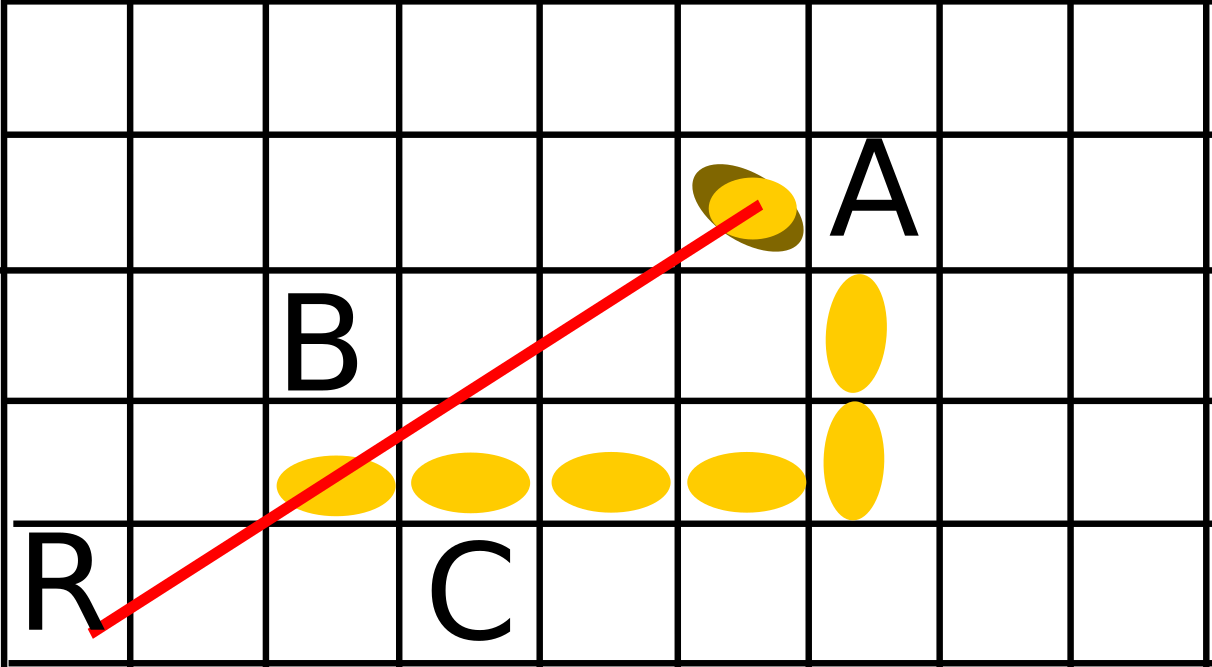
\includegraphics[width=70mm]{../img/ray_trace2.png}
	\caption{Image describing raytracing update. Yellow elipses represent normal distributions. Letter R represent robot position and red line ray tracing line. \gls{RCU} will be applied to the cell marked A. A distribution in cell marked with letter B will get updated as unoccupied. Cell C will stay without any update.}
	\label{fig:raytrace}
\end{figure}

\newpage   
\section{Registration algorithms}
\label{sec:reg_alg}
\subsection{NDT registration}
\label{subsec:P2D_NDT}
NDT registration process was first time explained by \cite{Biber03}. They have explained how to make 2D registration between older scan (target scan) and newer scan (source scan). Target scan was converted to NDT grid by technique mentioned in section \ref{subsec:NDT_grid}. Result of registration should be transformation defined in 2D:
\begin{equation}
T: 
\begin{pmatrix}
x' \\ y'
\end{pmatrix}
=
\begin{pmatrix}
\cos \theta  & -\sin \theta\\
\sin \theta & \cos \theta
\end{pmatrix}
\begin{pmatrix}
x \\ y
\end{pmatrix}
+
\begin{pmatrix}
t_{x} \\ t_{y} 
\end{pmatrix}
\end{equation}
where $ (t_{x},t_{y})^{T}$ represents translation and $\theta$ represents rotation. Transformation is used for transforming source scan. At the beginning of program parameters of transformation are initialized either by zero or from initial guess. For each point of transformed scan cost function is computed This function is defined as:
\begin{equation}
score(\textbf{p}) = \sum_{i}^{} \exp(-\frac{1}{2} ((T(x_{i},\textbf{p})- \mu_{i})^{T} P^{-1}_{i}   (T(x_{i},\textbf{p})- \mu_{i}) ) 
\end{equation}
where $\textbf{p} = (t_{x},t_{y}, \theta)$ are parameters of transformation, $N(\mu_{i},P_{i})$ are parameters of normal distribution where point $x$ is transformed by transformation $T$.Goal of the NDT scan-matching is to find parameters $\textbf{p}$ which maximize this function. This maximization problem is changed to minimization problem by searching for minimal value of -score. Newton's algorithm finds minimizing parameters in $p$ by iteratively solving equation 
\begin{equation}
 H \varDelta p = -g
\end{equation}  

Representation of hessian, gradient and all derivations might be found in work of \cite{magnusson09}. Magnusson also introduced new scaling parameters into score function in order to reject possible outliers. \gls{PDF} inside of cells of target \gls{NDT} grid may not be always from normal distribution. In practice any representation which approximates structure of the element is valid. Outliers are points far from the mean of distribution and cause unbounded growth of \gls{PDF}.

At the beginning, algorithm created discrete \gls{NDT} grid out of target scan. This introduces discretization problems. These problems are cause by points generating \gls{PDF} which are larger than their cells. In the original work of \cite{Biber03} this was solved by creating 4 target grids where each grid is translated by half of the cell size in single direction. This process made this algorithm inefficient. Introduction to multi-layer \gls{NDT} grid structure, presented by \cite{ulas20113d}, solved this problem. Multi-layer approach consists of several grids with different resolution. Grids are ordered from coarser grid to finer grid. Algorithm starts with coarse grid and estimates parameters of transformation. Calculated transformation is used as initial guess at lower level. This principle practically eliminated need for four overlapping grids. It also offered better convergence time and increase to robustness. Algorithm is able to converge when matched scans are farther away. Good configuration is 4 layers with cell sizes 2, 1, 0.5 and 0.25 meters. 

Another improvement to algorithm is usage of concept of linked cells. In practical registration very often part of the source scan lie far from any target cells. This causes only small portion of points contribute to score function. It can cause algorithm failure or just increase time of convergence. Linked cells prevent this by providing cells in target scan, which are close to the point from source scan. Implementation of this technique is possible with use of kD-tree with means of all cells as input points. Every point or source scan finds k-nearest cells and execute score calculation on them.

\begin{algorithm}
\label{alg:p2d_ndt}
    \caption{\gls{NDT} algortihms with muilti layer and linked cell enhancements}
\begin{algorithmic}[1]
 \Require source scan, target scan,  parameters $(x,y,\theta)$ of initial transformation, cell resolution for each layer
 \Function{NDTRegistration}{$scan_{s}$, $scan_{t}$, $p_{init}$,$resolutions$}
	 \State $\textbf{p} \gets p_{init}$
	 \ForAll{$res$ from $resolutions$}
		 \State $ndt_{t} \gets$createNDTGrid($res$,$scan_{t}$)
		 \Comment described in section \ref{subsec:NDT_grid}
		 \State transform each point $x_{i} \in scan_{trans}$ with $T(x_{i},\textbf{p})$
		 \State $\textbf{p} \gets$ computeSingleGrid($scan_{trans}$, $ndt_{t}$, $\textbf{p}$)
	 \EndFor
	 \State \Return calculated parameters $\textbf{p}$ of transformation
 \EndFunction
\end{algorithmic}
\end{algorithm}
\begin{algorithm}
\label{alg:p2d_ndt_single}
\caption{Computing transformation on with single target \gls{NDT} grid and source point cloud}
\begin{algorithmic}[1]
 \Require source scan, target NDT grid,  parameters $(x,y,\theta)$ of initial transformation
 \Function{computeSingleGrid}{$scan_{s}$, $ndt_{t}$,$p_{init}$}
	 \While {not converged}
		 \State $\textbf{p} \gets p_{init}$
		 \State $(score, g,H) \gets (0,0,0)$
		 \ForAll {points $x_{i} \in scan_{trans}$}
			 \State $\bar{x_{i}} \gets T(x_{i},\textbf{p})$
			 \State $cells \gets $find k-closest cells to $\bar{x_{i}} $
			 \ForAll{cells $c_{i} \in cells$}
			 \State \{based on \cite{magnusson09}\}
				 \State $(score,g,H) \gets (score,g,H)  + $ calcNewtonParameters($c_{i}$,$\bar{x_{i}}$)
			 \EndFor 
		 \EndFor
		 \State solve $H\varDelta p = - g$
		 \State $\textbf{p} \gets \textbf{p} + \varDelta p$
	 \EndWhile
	 \State \Return $\textbf{p}$
 \EndFunction
\end{algorithmic}
\end{algorithm}
         
 

\subsection{D2D-NDT registration}
\label{subsec:D2D_NDT}
\gls{D2D}-\gls{NDT} is variant of \gls{NDT} registration algorithm proposed by \cite{Stoyanov01102012}. It is extension of original algorithm presented in section \ref{subsec:P2D_NDT}. Instead of using only one grid for target scan. This aproach uses two grids. One for source scan and second for target grid. Algorithm than minimize the sum of $L_{2}$ distances between pairs of \gls{PDF}'s from both grids. Formally, transformation between two sets of cells $X$ and $Y$ is defined as:
\begin{equation}
f(\textbf{p}) = \sum_{i = 1, j =1}^{n_{X}, n_{Y}} -d_{1}\exp\left( - \frac{d_{2}}{2}  \mu_{ij}^{T}(R^{T}P_{i}R + P_{j})^{-1} \mu_{ij} \right)
\end{equation}
\begin{equation}
\label{eq:D2D_2}
\mu_{ij} = R\mu_{i} + t - \mu_{j}
\end{equation}
where $\textbf{p} = (t_{x},t_{y},\theta)$; $X(\mu_{i},P_{i})$ and $Y(\mu_{j}, P_{j})$ are \gls{PDF}'s of individual cells in pair; a pair $(R,t)$ represents rotation matrix from parameter $\theta$ and translation vector $t=(t_{x},t_{y})$. Regulation parameters d1 and d2 are set to values $d_{1} = 1$ and $d_{2}=0.05$. Equation \ref{eq:D2D_2} represents difference in means where mean $u_{i}$ is transformed to new position.

Optimization of this function is done in similar way to \ref{subsec:P2D_NDT}  by utilizing Newtons method and solving $H\varDelta \textbf{p} = -g$. Derivations for calculation of hessian and gradient are presented in work of \cite{Stoyanov01102012}.

This algorithm is also possible to improve by iterating over multiple layers with different resolutions similar to \gls{NDT} registration in previous section.

In comparison, with \gls{NDT} registration this algorithm needs only \gls{NDT} grids for registration. Point cloud can be thrown away after successful creation of grid. This allow saving memory and efficiently represent maps in \gls{SLAM}. In addition, \gls{D2D} is almost ten times faster than standard \gls{NDT} registration on same dataset. This was proven in comparative study from \cite{NDTcomparative}. The main cause of this speed up is smaller number of calls for score calculation. In \gls{P2D}-\gls{NDT} mentioned in last section we need to calculate score for each point in source point cloud. In case of \gls{D2D} we just calculate score function for each cell of source grid. This is done by generating only pairs between cell from source grid and closest cell from target cell. Closest cell can be easily found by using kD-tree with values of target grid's means.
  
\newpage
\subsection {ICP}
\label{subsec:ICP}
The iterative closest point (\gls{ICP}) algorithm was first introduced by \cite{chen92ICP} and it is still very popular method for registering point clouds. To briefly summaries algorithm: ICP iteratively refines position of two point clouds by optimizing the sum of square distances between corresponding pair of points from two clouds. This approach is usually called point-to-point registration. Class of algorithms based on \gls{ICP} has developed many modifications. Surrvey of base type of ICP algorithms and their comparison on well designed datasets is in work of \cite{pomerleau2013comparing}. 



\subsection{Correlative scan registration}
\label{subsec:Corr}
Correlative scan registration is algorithm presented by \cite{olson2009real}. This method was developed to robustly solve registration problem. It does not require any initial guess. Therefore, it is possible to use it for loop closure registration.

 The algorithm requires two point clouds. Target point cloud is used for generation of fast look up table filled with bit values. It is created by separating points from target cloud into individual cells. Every cell which has some points in it is marked as occupied. After this step we have a table with value 1 in cells with some points and value 0 in cells without points. In next step we add sensor noise to the table. As a function of our noise we use radially symmetric kernel. 
 \begin{equation}
 \label{eq:smooth_kernel}
 K_{i,j} = \exp\left(\frac{-1}{2}\left(\frac{\sqrt{(i r)^{2} + (j r)^{2}}}{\sigma}\right)^{2}\right) \eta
 \end{equation}
 \begin{equation}
 K =
 \begin{pmatrix}
  2 & 14 & 2\\
  14 & 100 & 14 \\
  2 & 14 & 2 
 \end{pmatrix}
 \end{equation}
 where $K_{i,j}$ is one element of kernel; $\sqrt{(i r)^{2} + (j r)^{2}}$ is euclidean distance from center of the kernel to the element $i,j$ with cell size parameter $r$. Standard deviation of sensor nose is abbreviated by $\sigma$ and $\eta$ is kernels max value.

 The Kernel overlaps over every occupied cell in the table. If value of kernel is higher than value in table. Table is updated with the kernels value. Generated smoothing can be seen in figure \ref{fig:kernel}. 
 
 This algorithm is avoiding initial guess by trying all possible rotations and translations of source cloud. Every point of transformed source cloud is mapped into certain cell of look up table. The total score of transformed cloud is sum of all mapped cells scores. Algorithm usually tries rotations and translations from selected range. Transformation with the best score is the most probable transformation.
 
 This brute force process might take long time if we select small cell size to achieve good registration. To speed up this process we first need to avoid computationally expensive calculation of goniometric functions in transformation. This can be achieved by first generating all possible rotations of point cloud. For each rotation we try all translations from selected range with step size selected based on cell size of look up table.
 
 Real speed improvements offers usage of two layer architecture of look up tables. The first table has coarse resolution. This table is used for initial estimation on the whole range of selected rotations and translations. The transformations with best score are used in the second round. From every good transformation is generated search space voxel. Origin of voxel is taken from transformation. Size of voxel is cell size from coarse table. Search voxels are evaluated on look up table with fine resolution. Search space is this time limited to search voxel and initial transformation is taken from origin of voxel. The best result is our solution. By this process computation time drops rapidly as show in work of \cite{olson2009real}.     
   \begin{figure}
   \label{fig:kernel}
   	\centering
   	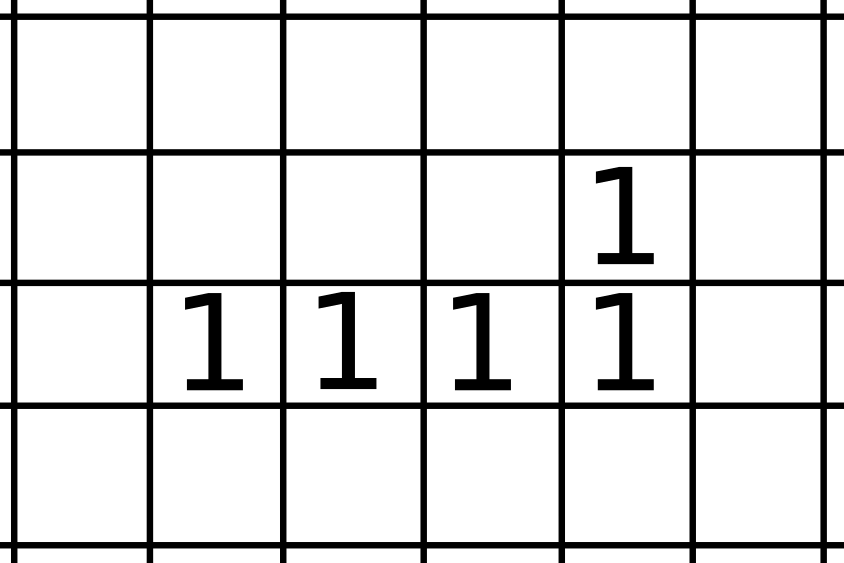
\includegraphics[width=50mm]{../img/kernel_a.png}
   	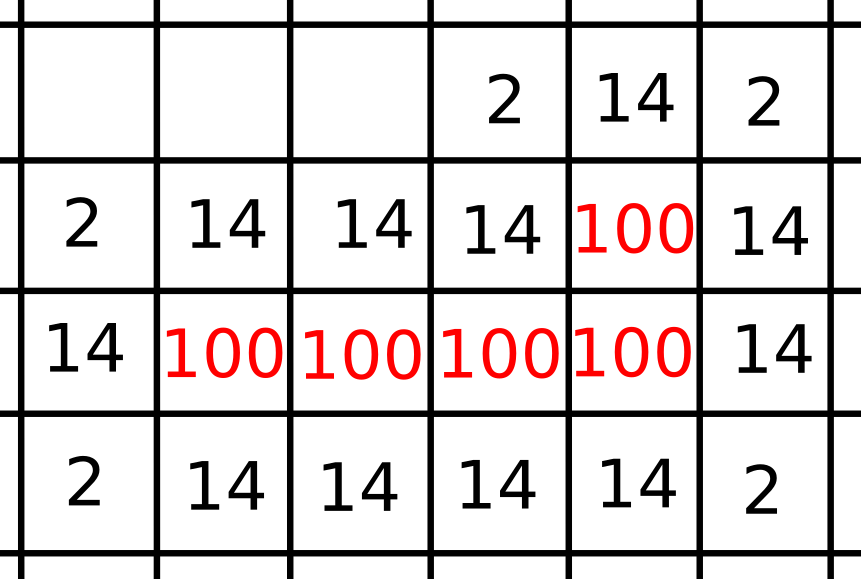
\includegraphics[width=50mm]{../img/kernel_b.png}
   	
   	\caption{Image on the left shows look up table before applying smoothing kernel. Image on the right is after application of kernel.}
   	\label{fig:raytrace}
   \end{figure} 
\newpage
     

